\documentclass[12pt]{article}
\usepackage[utf8]{inputenc}
\usepackage{float}
\usepackage{amsmath}
\usepackage{amssymb}
%\usepackage{alltt}
\usepackage[dvips]{graphicx}
%\usepackage{a4wide}
\usepackage{epsfig}
\usepackage{fancybox}
\usepackage{verbatim}
\usepackage{array}
\usepackage{latexsym}
\usepackage{alltt}
%\usepackage{dsfont}
\usepackage{caption}
\usepackage{subcaption}
%\usepackage{fullpage}
\usepackage{hyperref}
\usepackage{textcomp}
\usepackage{listings}
\usepackage{color}
\usepackage{amsmath}
\usepackage{amsfonts}
\usepackage{tikz}
\usepackage{float}
\usepackage{booktabs}
\usepackage{ifthen}

\usepackage[hmargin=3cm,vmargin=6.0cm]{geometry}
%\topmargin=0cm
\topmargin=-2cm
\addtolength{\textheight}{6.5cm}
\addtolength{\textwidth}{2.0cm}
%\setlength{\leftmargin}{-5cm}
\setlength{\oddsidemargin}{0.0cm}
\setlength{\evensidemargin}{0.0cm}

%misc libraries goes here



\begin{document}

\section*{Student Information } 
%Write your full name and id number between the colon and newline
%Put one empty space character after colon and before newline
Full Name : YAHYA SUNGUR \\
Id Number : 2375723 \\
.
% Write your answers below the section tags
\section*{Answer 1}
\paragraph{a-)}.\\
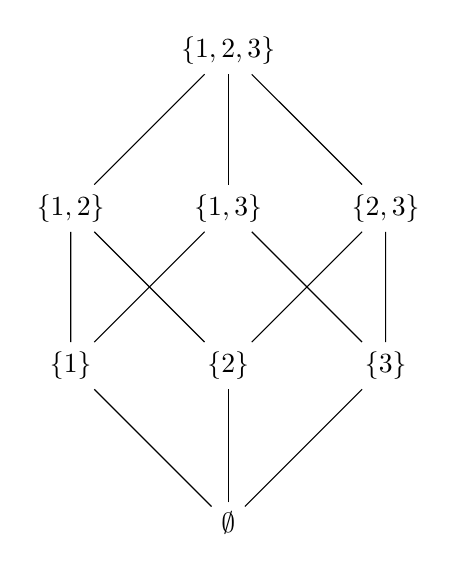
\begin{tikzpicture}
    \node (123) at (4,0) {$\{1,2,3\}$};
    \node (12) at (2,-2)  {$\{1,2\}$};
    \node (13) at (4,-2) {$\{1,3\}$};
    \node (23) at (6,-2) {$\{2,3\}$};
    \node (1) at (2,-4)  {$\{1\}$};
    \node (2) at (4,-4) {$\{2\}$};
    \node (3) at (6,-4) {$\{3\}$};
    \node (empty) at (4,-6) {$\emptyset$};
    \draw (empty)--(1)--(12)--(123)--(23)--(3)--(empty);
    \draw (1)--(13)--(3);
    \draw (123)--(13);
    \draw (12)--(2)--(23);
    \draw (empty)--(2);
\end{tikzpicture}
\paragraph{b-)}
Let X and Y be two subsets of A. The least upper bound and the greatest lower bound of X and Y are X $\cup$ Y and X $\cap$ Y, respectively. Hence, (P (A),$\subseteq$) is a lattice.
\paragraph{c-)}
Since \{1,2,3\} are not succeeded by another element. It is the maximal element.
\paragraph{d-)}
Since $\emptyset$ are not preceded by another element. It is the minimal element.
\paragraph{e-)}
The set A is the greatest element in this poset, because $T \subseteq A$ whenever T is a subset of A.
\paragraph{f-)}
The least element is the empty set, because $\emptyset \subseteq T$ for any subset T of A.
\paragraph{g-)}.\\
Upper bounds of \{1\} are \{1,3\},\{1,2\},\{1,2,3\} and Least Upper Bounds of \{1\} are \{1,3\} and \{1,2\} \\
Upper bounds of \{3\} are \{1,3\},\{2,3\},\{1,2,3\} and Least Upper Bounds of \{3\} are \{1,3\} and \{2,3\}
\section*{Answer 2}
\paragraph{a-)}
deg(a) = 2, deg(b) = 4, deg(c) = 2, deg(d ) = 3, deg(e) = 3 \\
Sum = 14
\paragraph{b-)}
\[
    \begin{pmatrix}
        0 & 1 & 0 & 0 & 1 \\
        1 & 0 & 1 & 1 & 1 \\
        0 & 1 & 0 & 1 & 0 \\
        0 & 1 & 1 & 0 & 1 \\
        1 & 1 & 0 & 1 & 0 \\
    \end{pmatrix}
\]
So, number of non-zero entries in the adjacency matrix is 14
\paragraph{c-)}
\[
    \begin{pmatrix}
        1 & 1 & 0 & 0 & 0 & 0 & 0 \\
        1 & 0 & 1 & 0 & 0 & 0 & 0 \\
        0 & 0 & 0 & 0 & 1 & 1 & 0 \\
        0 & 0 & 0 & 0 & 0 & 1 & 1 \\
        0 & 0 & 0 & 1 & 1 & 0 & 1 \\
        0 & 1 & 1 & 1 & 0 & 0 & 0 \\
    \end{pmatrix}
\]
So, number of non-zero entries in the incidence matrix is 14
\paragraph{d-)}
Yes,\\
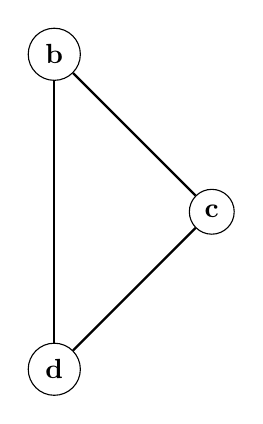
\begin{tikzpicture}
	\node[shape=circle,draw=black] (b) at (4, 4)     {\textbf{b}};
	\node[shape=circle,draw=black] (c) at (6, 2)     {\textbf{c}};
	\node[shape=circle,draw=black] (d) at (4, 0)     {\textbf{d}};

	\path[-, thick] (b) edge (c);
	\path[-, thick] (b) edge (d);
	\path[-, thick] (d) edge (c);
\end{tikzpicture} 
\paragraph{e-)}
It is not a bipartite graph. And, this subgraph of G is a bipartite graph.\\
	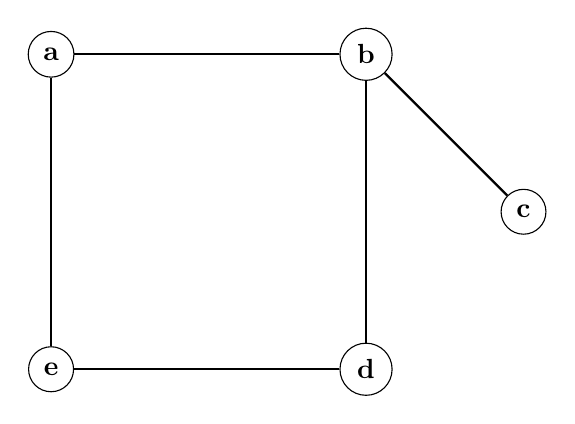
\begin{tikzpicture}
	
	\node[shape=circle,draw=black] (a) at (0, 4)     {\textbf{a}};
	\node[shape=circle,draw=black] (b) at (4, 4)     {\textbf{b}};
	\node[shape=circle,draw=black] (c) at (6, 2)     {\textbf{c}};
	\node[shape=circle,draw=black] (d) at (4, 0)     {\textbf{d}};
	\node[shape=circle,draw=black] (e) at (0, 0)     {\textbf{e}};
	
	\path[-, thick] (a) edge (b);
	\path[-, thick] (a) edge (e);
	\path[-, thick] (b) edge (c);
	\path[-, thick] (b) edge (d);
	\path[-, thick] (d) edge (e);
	
	\end{tikzpicture} 
\paragraph{f-)}
There are 7 edges, and each of them can have three different possibilities. The sample has 3 different directional conditions for a and b. from a to b, b to a, and both at the same time. So, there are $3^7 = 2187$ directed graphs that have G as their underlying undirected graph.
\paragraph{g-)}
Simple path is a path that does not contain an edge more than once, and the simple longest path in G can be obtained by constructing Euler Path. \\ For example, (d,c,b,a,e,d,b,e) which has 7 edges. \\
Hence, the length of the simple longest path in G = 7
\paragraph{h-)}
An undirected graph is called  connected if there is a path between every pair of vertices.And, graph G is connected. So, it has only one connected components which is itself.
\paragraph{i-)}
By the theorem, a connected multigraph with at least two vertices has an Euler circuit if and only if each of its vertices has an even degree. But, G has two vertices of odd degree (d,e). So, there is no Euler circuit.
\paragraph{j-)}
By the theorem,a graph with an Euler path has exactly two vertices of odd degree. And, since G has exactly two vertices of odd degree (d,e). So it has a Euler path, which is (d,c,b,a,e,d,b,e).  
\paragraph{k-)}
Yes, (a,b,c,d,e,a)
\paragraph{l-)}
Yes, (a,b,c,d,e)
\section*{Answer 3}
\begin{figure}[h]
    \begin{center}
        \includegraphics[width=.4\textwidth]{Capture.JPG}
    \end{center}
    \label{my_fig}
\end{figure}
The function f with f(a) = a', f(b) = c', f(c) = e', f(e) = b', f(f) = h', f(h) = f', f(g) = d' is a one-to-one correspondence between G and H. And according to the figure above, adjacent vertices for all vertex in G correspond to the adjacent vertices for all vertex in H appropriately. So, G and H are isomorphic.
\section*{Answer 4}
Let G = (V,E,w), V: vertices, E: edges, w: weights\\
Let T be a set which T $\subseteq$ V with a $\notin$ T (a is the start vertices of path), and Let P be a set which P $\subseteq$ V-T \\
and also, let l(t) = w(\{a,t\})\\.\\
First step:\\
P = {a} $\implies$ l(b) = 3, l(e) = 5, l(h) = 4. and l(c)=l(f)=l(i)=l(d)=l(g)=l(j)=l(k)= $\infty$\\
current shortest paths: ab:3 , ae:5 , ah:4\\.\\
Second step:(take shortest (b))\\
P = {a,b} $\implies$ l(e) = 8, l(f) = 10, l(c) = 5. and l(i)=l(d)=l(g)=l(j)=l(k)= $\infty$\\
current paths: abe:8 , abf:10, abc:5 and Since ae < abe no update\\
current shortest paths: abf:10, abc:5 , ae:5\\.\\
Third step:(take shortest (c)\\
P = {a,b,c} $\implies$ l(d) = 8, l(g) = 11, l(f) = 7. and l(i)=l(j)=l(k)=$\infty$\\
current paths: abcd:8 , abcg:11, abcf:7 and Since abcf < abf ,updated\\
current shortest paths: abcd:8 , abcg:11, abcf:7\\.\\
Fourth step: (take shortest (f))\\
P = {a,b,c,f} $\implies$ l(i) = 11, l(g) = 11, l(j) = 10. and l(k)=$\infty$\\
current shortest paths: abcfi:11 , abcfg:11, abcfj:10\\.\\
Last step: (take shortest (j))\\
It is a destination point. So the shortest path is\\
a-b-c-f-j and its length is 10.
\section*{Answer 5}
By using Prim's Algorithm,
\begin{table}[H]
    \begin{center}
        \begin{tabular}{|l|c|r|}
             \toprule
             Choice & Edge & Weight\\
             \midrule
             1 & \{a,b\} & 1 \\
             \midrule
             2 & \{a,d\} & 3 \\
             \midrule             
             3 & \{b,c\} & 4 \\
             \midrule
             4 & \{c,f\} & 2 \\
            \midrule
             5 & \{f,e\} & 2 \\
            \bottomrule
        \end{tabular}
    \end{center}
\end{table}
\paragraph{b-)}
\begin{figure}[H]
	\centering
	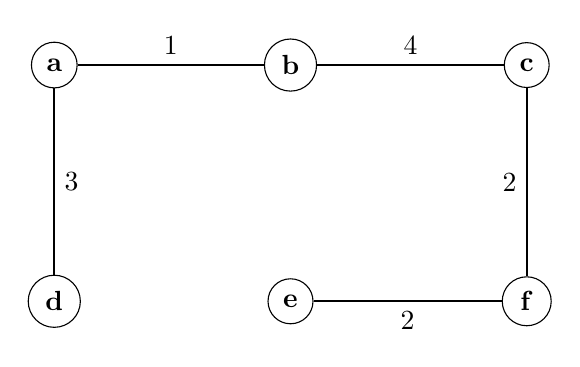
\begin{tikzpicture}
	
	\node[shape=circle,draw=black] (a) at (0, 3)     {\textbf{a}};
	\node[shape=circle,draw=black] (b) at (3, 3)     {\textbf{b}};
	\node[shape=circle,draw=black] (c) at (6, 3)     {\textbf{c}};
	\node[shape=circle,draw=black] (d) at (0, 0)     {\textbf{d}};
	\node[shape=circle,draw=black] (e) at (3, 0)     {\textbf{e}};
	\node[shape=circle,draw=black] (f) at (6, 0)     {\textbf{f}};
	
	\path[-, thick] (a) edge node[above]{1} (b);
	\path[-, thick] (b) edge node[above]{4} (c);
	\path[-, thick] (a) edge node[right]{3} (d);
	\path[-, thick] (c) edge node[left]{2} (f);
	\path[-, thick] (e) edge node[below]{2} (f);
	
	\end{tikzpicture} 
\end{figure}
\paragraph{c-)}.\\
For this case, minimum spanning tree is not unique. For example, following is another minimum spanning tree.
\begin{figure}[H]
	\centering
	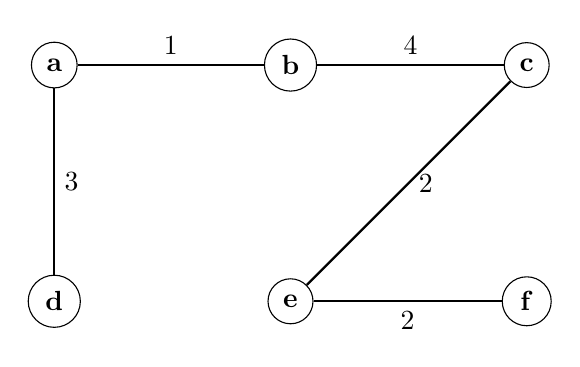
\begin{tikzpicture}
	
	\node[shape=circle,draw=black] (a) at (0, 3)     {\textbf{a}};
	\node[shape=circle,draw=black] (b) at (3, 3)     {\textbf{b}};
	\node[shape=circle,draw=black] (c) at (6, 3)     {\textbf{c}};
	\node[shape=circle,draw=black] (d) at (0, 0)     {\textbf{d}};
	\node[shape=circle,draw=black] (e) at (3, 0)     {\textbf{e}};
	\node[shape=circle,draw=black] (f) at (6, 0)     {\textbf{f}};
	
	\path[-, thick] (a) edge node[above]{1} (b);
	\path[-, thick] (b) edge node[above]{4} (c);
	\path[-, thick] (a) edge node[right]{3} (d);
	\path[-, thick] (c) edge node[right]{2} (e);
	\path[-, thick] (e) edge node[below]{2} (f);
	
	\end{tikzpicture} 
\end{figure}
\section*{Answer 6}
\paragraph{a-)}
number of vertices = 13 \\
number of edges = 12 \\
height of T = 4 
\paragraph{b-)}
w - s - m - t - q - x - n - y - u -  z - v - r - p
\paragraph{c-)}
w - s - q - m - t - p - x - u - n - y - r - z - v 
\paragraph{d-)}
p - q - s - w - t - m - r - u - x - y - n - v - z
\paragraph{e-)}
A full binary tree is a tree in which every node other than the leaves has two children. So, T is not a full binary tree, because s,t,y and v have only one child.
\end{document}